\documentclass[tikz,border=0pt]{standalone}
\usepackage{xcolor}
\definecolor{acid}{HTML}{B8E04A}
\definecolor{amber}{HTML}{FFB23E}
\definecolor{badge}{HTML}{262238}
\definecolor{badgehi}{HTML}{3A3454}
\definecolor{coral}{HTML}{FF7B66}
\definecolor{crystal}{HTML}{6E8FB0}
\definecolor{faunateal}{HTML}{3B8C88}
\definecolor{faunatealhi}{HTML}{5BB3A9}
\definecolor{flesh}{HTML}{C98FA8}
\definecolor{gold}{HTML}{FFC93C}
\definecolor{goldhi}{HTML}{FFE9A0}
\definecolor{ground}{HTML}{2D2939}
\definecolor{groundB}{HTML}{322E40}
\definecolor{groundC}{HTML}{29253A}
\definecolor{gunmetal}{HTML}{565D6C}
\definecolor{gunmetaldark}{HTML}{383D49}
\definecolor{hazard}{HTML}{F2C230}
\definecolor{haze}{HTML}{6B4473}
\definecolor{heal}{HTML}{FF5C70}
\definecolor{ink}{HTML}{14111C}
\definecolor{moon}{HTML}{B9A8C9}
\definecolor{offwhite}{HTML}{E3DFD0}
\definecolor{olive}{HTML}{7D8740}
\definecolor{olivehi}{HTML}{A2AD5A}
\definecolor{pebble}{HTML}{3B3650}
\definecolor{rift}{HTML}{7F45E8}
\definecolor{rifthi}{HTML}{D3B1FF}
\definecolor{rock}{HTML}{4B4562}
\definecolor{rockdark}{HTML}{36314A}
\definecolor{rockhi}{HTML}{5D5677}
\definecolor{sensor}{HTML}{FF4A5C}
\definecolor{shadow}{HTML}{1D1A28}
\definecolor{shot}{HTML}{FF3DCF}
\definecolor{shothi}{HTML}{FFC4F1}
\definecolor{sky}{HTML}{2A2245}
\definecolor{skyhi}{HTML}{1E1A33}
\definecolor{skylow}{HTML}{4A3260}
\definecolor{suit}{HTML}{F2F5F7}
\definecolor{suitshade}{HTML}{BFCBD6}
\definecolor{teal}{HTML}{33D1BF}
\definecolor{ticket}{HTML}{B48CFF}
\definecolor{violet}{HTML}{8462B8}
\definecolor{violetdark}{HTML}{5B4284}
\definecolor{violethi}{HTML}{A68AD6}
\definecolor{visor}{HTML}{1D2B3E}
\definecolor{visorhi}{HTML}{9DE6F4}
\definecolor{weakspot}{HTML}{E8F25A}
\definecolor{xp}{HTML}{4FEFFF}
\definecolor{xphi}{HTML}{D2FBFF}
\newlength{\Ink}\setlength{\Ink}{3pt}
\tikzset{inked/.style={draw=ink,line width=\Ink,line join=round,line cap=round}}
\begin{document}
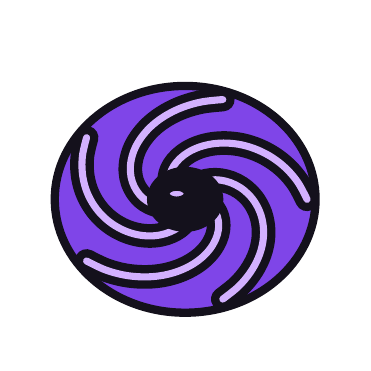
\begin{tikzpicture}
\useasboundingbox (0,0) rectangle (4,4);
\clip (0,0) rectangle (4,4);
\filldraw[inked,fill=rift] (2,1.82) ellipse (1.656 and 1.44);
\draw[draw=ink,line width=8.561pt,line cap=round,line join=round] plot[smooth, tension=0.6] coordinates {(3.548,1.82) (3.436,2.029) (3.289,2.205) (3.115,2.345) (2.925,2.446) (2.729,2.509) (2.534,2.534) (2.351,2.525) (2.186,2.486) (2.045,2.422) (1.934,2.339) (1.855,2.245) (1.81,2.146) (1.798,2.049) (1.816,1.961)};
\draw[draw=rifthi,line width=2.561pt,line cap=round,line join=round] plot[smooth, tension=0.6] coordinates {(3.548,1.82) (3.436,2.029) (3.289,2.205) (3.115,2.345) (2.925,2.446) (2.729,2.509) (2.534,2.534) (2.351,2.525) (2.186,2.486) (2.045,2.422) (1.934,2.339) (1.855,2.245) (1.81,2.146) (1.798,2.049) (1.816,1.961)};
\draw[draw=ink,line width=8.561pt,line cap=round,line join=round] plot[smooth, tension=0.6] coordinates {(2.478,3.087) (2.213,3.058) (1.971,2.99) (1.762,2.89) (1.588,2.765) (1.456,2.623) (1.364,2.472) (1.315,2.32) (1.304,2.174) (1.329,2.042) (1.384,1.929) (1.462,1.838) (1.557,1.775) (1.661,1.739) (1.765,1.732)};
\draw[draw=rifthi,line width=2.561pt,line cap=round,line join=round] plot[smooth, tension=0.6] coordinates {(2.478,3.087) (2.213,3.058) (1.971,2.99) (1.762,2.89) (1.588,2.765) (1.456,2.623) (1.364,2.472) (1.315,2.32) (1.304,2.174) (1.329,2.042) (1.384,1.929) (1.462,1.838) (1.557,1.775) (1.661,1.739) (1.765,1.732)};
\draw[draw=ink,line width=8.561pt,line cap=round,line join=round] plot[smooth, tension=0.6] coordinates {(0.748,2.603) (0.696,2.376) (0.694,2.158) (0.737,1.956) (0.82,1.778) (0.935,1.627) (1.073,1.509) (1.226,1.424) (1.384,1.373) (1.54,1.355) (1.685,1.368) (1.812,1.407) (1.916,1.466) (1.993,1.541) (2.038,1.624)};
\draw[draw=rifthi,line width=2.561pt,line cap=round,line join=round] plot[smooth, tension=0.6] coordinates {(0.748,2.603) (0.696,2.376) (0.694,2.158) (0.737,1.956) (0.82,1.778) (0.935,1.627) (1.073,1.509) (1.226,1.424) (1.384,1.373) (1.54,1.355) (1.685,1.368) (1.812,1.407) (1.916,1.466) (1.993,1.541) (2.038,1.624)};
\draw[draw=ink,line width=8.561pt,line cap=round,line join=round] plot[smooth, tension=0.6] coordinates {(0.748,1.037) (0.981,0.926) (1.221,0.859) (1.458,0.835) (1.682,0.849) (1.886,0.898) (2.063,0.976) (2.207,1.075) (2.315,1.189) (2.387,1.311) (2.422,1.432) (2.422,1.546) (2.391,1.647) (2.335,1.728) (2.259,1.787)};
\draw[draw=rifthi,line width=2.561pt,line cap=round,line join=round] plot[smooth, tension=0.6] coordinates {(0.748,1.037) (0.981,0.926) (1.221,0.859) (1.458,0.835) (1.682,0.849) (1.886,0.898) (2.063,0.976) (2.207,1.075) (2.315,1.189) (2.387,1.311) (2.422,1.432) (2.422,1.546) (2.391,1.647) (2.335,1.728) (2.259,1.787)};
\draw[draw=ink,line width=8.561pt,line cap=round,line join=round] plot[smooth, tension=0.6] coordinates {(2.478,0.553) (2.675,0.711) (2.825,0.888) (2.928,1.075) (2.984,1.262) (2.995,1.443) (2.966,1.61) (2.902,1.756) (2.811,1.877) (2.699,1.97) (2.576,2.032) (2.448,2.064) (2.325,2.066) (2.214,2.042) (2.122,1.995)};
\draw[draw=rifthi,line width=2.561pt,line cap=round,line join=round] plot[smooth, tension=0.6] coordinates {(2.478,0.553) (2.675,0.711) (2.825,0.888) (2.928,1.075) (2.984,1.262) (2.995,1.443) (2.966,1.61) (2.902,1.756) (2.811,1.877) (2.699,1.97) (2.576,2.032) (2.448,2.064) (2.325,2.066) (2.214,2.042) (2.122,1.995)};
\filldraw[inked,fill=ink] (2,1.82) ellipse (0.432 and 0.36);
\filldraw[inked,fill=rifthi] (1.892,1.892) ellipse (0.144 and 0.09);
\end{tikzpicture}
\end{document}
